\chapter[Planificación]{
  \label{chp:plan}
  Planificación
}
\minitoc
\newpage

Neste capítulo explicarase a planificación do traballo realizado e a avaliación de custes.  

\section{Iteracións}

Como se explicou no capítulo \ref{chp:metodoloxia}, o desenvolvemento executouse de  de forma iterativa e incremental onde unha iteración son os obxectivos a cumprir entre dúas reunións co cliente. Ao ser isto un proxecto de final de carreira, contarase o tempo entre as sesións de revisión de progresos entre o director do proxecto e o alumno.

\subsection{Reunión inicial}

Produciuse un encontro con membros de Cuac FM (a radio comunitaria da Coruña) e a URCM onde se entrou en contacto cos usuarios finais do proxecto a realizar. A URCM (Unión de Radios Comunitarias de Madrid) está composta por unha serie de emisoras independentes e con programas de seu; todos eles listados nunha sección da web (ver figura \ref{fig:urcm}) que á súa vez da acceso ao directorio dos ficheiros de audio (aos que a partir de agora nos referiremos coma \say{audios}) publicados por ditas emisoras. Esta sección da web, pese a súas limitacións, leva funcionando uns anos e resultou ser moi positiva para a redifusión dos programas por distintos colectivos.

\begin{figure}[h]
	\centering
	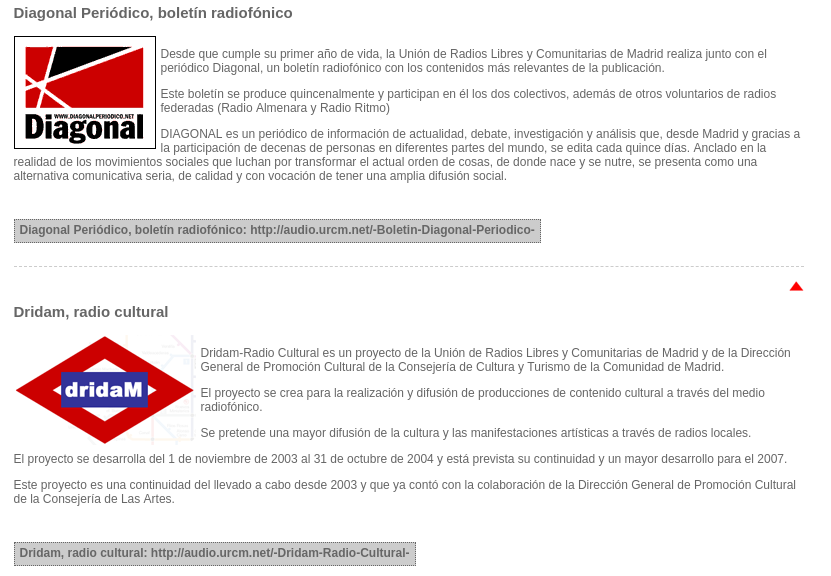
\includegraphics[scale=0.55,keepaspectratio=true]{./images/urcm.png}
	\caption{Sección de audios da web da URCM que inspira o proxecto.}
	\label{fig:urcm}
\end{figure}

Inspirados nesta idea, propúxose crear unha ferramenta semellante, esta vez para a ReMC (Red de medios comunitarios), unha federación de medios comunitarios do Estado Español. Definíronse uns requirimentos iniciais, máis centrados naquel entón na
redifusión e a organización que na escoita.

\subsubsection{Requirimentos primitivos}

A seguinte lista é unha transcrición das notas tomadas durante esa primeira reunión:

\begin{itemize}
	\item Os usuarios dos sistema son as propias emisoras.
	\item As emisoras teñen que poder engadir audios.
	\item As emisoras poden acceder aos audios das outras.
	\item As emisoras teñen que poder saber quen está a emitir os seus programas.
\end{itemize}


